
%In this section is shown the architecture of the ProLine-RM as well as an description of its components. 
In Figure~\ref{fig:architecture} is depicted the architecture of the CrossFIRE. As shown in this figure, we devised the CrossFIRE on the top of the Eclipse Platform. On the other hand, both the RRM and RM have been developed using Eclipse Modeling Framework and Graphical Modeling Framework\footnote{http://www.eclipse.org/modeling/gmp/}. Moreover, we have studied FeatureIDE's source code and extended it in order to use for CF/CFF, its feature model editor and its configuration file, which is used to extract member of a CFF.

%The formal definition of both models is specified by a single metamodel, which due space limitation is now showed in this paper. This metamodel is a set of enumeration and metaclasses, which are either concrete or abstract. The metamodel was built based on the vocabulary commonly used in the context of CFs. Among these concepts, there are pointcuts, classifier extensions, method overriding, values and variabilities selections. We have studied the source code of the FeatureIDE and extended it to use for CF and its feature model editor.

As can be seen in Figure~\ref{fig:architecture}, all artifacts (source code, feature model, RM and RRM) that the CrossFIRE provides are persisted in a database. These artifacts are persisted in a remote server, available to be reused in the AE phase. This remote server is a physical computer, which is dedicated to run the RESTful API. Therefore, to send these artifacts by the server we have used this API as web service to cache the representation of all artifacts. This server receives requests of the CrossFIRE through RESTful, processes database queries and sends a response to the CrossFIRE by using RESTful as well. Furthermore, we have used Java Persistence API (JPA) 2.0 to deal with the way relational data is mapped to Java objects. To implement the database of the server, the MySQL was chosen.


%\begin{itemize}
%\item \textbf{Eclipse Plaform}: We have devise the CrossFIRE on the top of the Eclipse Platform, i.e., it has been developed using Eclipse Plug-In. The models RRM and RM have been developed using Eclipse Modeling Framework and Graphical Modeling Framework\footnote{http://www.eclipse.org/modeling/gmp/}%~\cite{GMP}. %It is a generic framework aiming to provides the ``plumbing'' that, before, every developer had to write themselves-salving state, connecting actions to menu items, toolbar items and keyboard shortcuts, window management, etc. 
	%\begin{itemize}
	%	\item \textbf{Workspace}: The workspace is a directory hierarchy containing 	both user files such as projects, source code, feature model, etc.
	%	\item \textbf{Workbench}: The workbench provides the overall structure and 
	%	presents an extensible user interface. It is built from two toolkits:   
	%		\begin{itemize}
	%			\item \textbf{The Standard Widget Toolkit (SWT)}: The SWT provides a common operating system independent API (Application Programming Interface) for widgets and graphics implemented in a way that allows tight integration with the underlying native window system. 
	%			\item \textbf{JFace}: It is an API that implements SWT in order to simplifies common user interface tasks.   
	%		\end{itemize}
	%	\item \textbf{Help}: It provides a full documentation of the ProLine-RM. For example, it supplies a help style documentation in order to guide the user use the ProLine-RM.
	%\end{itemize}
%\item \textbf{FeatureIDE}: We have studied its source code and extended it in order to use for CF and its feature model editor~\cite{Weiss:1999:SPE:317887}.
%\item \textbf{Web Service}: We have used RESTful as web service to cache the representation of the CF artifacts (e.g., feature models, source codes and `Reuse Model') in order to improve the CrossFIRE performance.
%\item \textbf{Server}: We have used a physical computer, which is dedicated to running the RESTful web services. It receives requests of the CrossFIRE through RESTful API, processes database queries and sends a response to the CrossFIRE using RESTful API as well.
%\item \textbf{JPA}: We have used Java Persistence API (JPA) 2.0 to deal with the way relational data is mapped to Java objects. 
%\item \textbf{DataBase}: To implement the database of the Server, the MySQL was chosen.
%\end{itemize}   

\begin{figure}[!h]
\centering
  % Requires \usepackage{graphicx}
 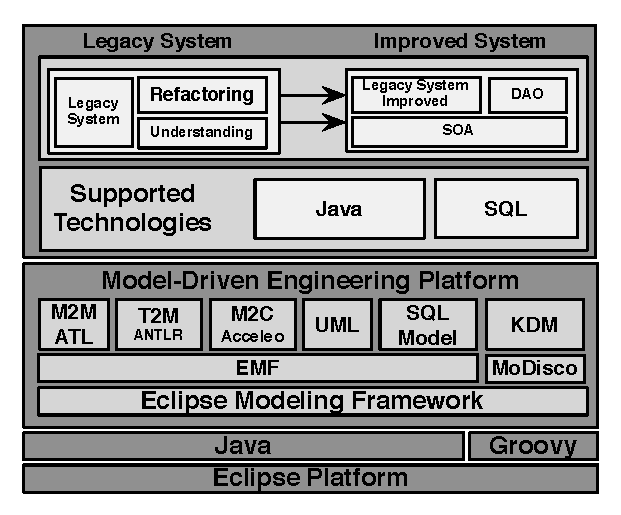
\includegraphics[scale=0.8]{Figuras/Arquitetura_da_Ferramenta}
\caption{Architecture of CrossFIRE}
\label{fig:architecture}
\end{figure}